\chapter{Technologien für Windows Desktop-Anwendungen}
\label{chap:TechnologienfürWindowsDesktop-Anwendungen}

\section{GUI-Framework}

Um eine Windows-Desktop-App zu erstellen gibt es sogenannte GUI-Frameworks/-Toolkits. Diese ermöglichen dem Programmierer mit einem Designer und vorgefertigten Elementen eigene Programme im Stil von Windows zu kreieren. 
Viele Designer besitzen auch einen sogenannten Layout-Manager mit dem das Erstellen von aufwendigen designten Programmen möglich wird. 
\\
\begin{figure}[H]
    \centering
    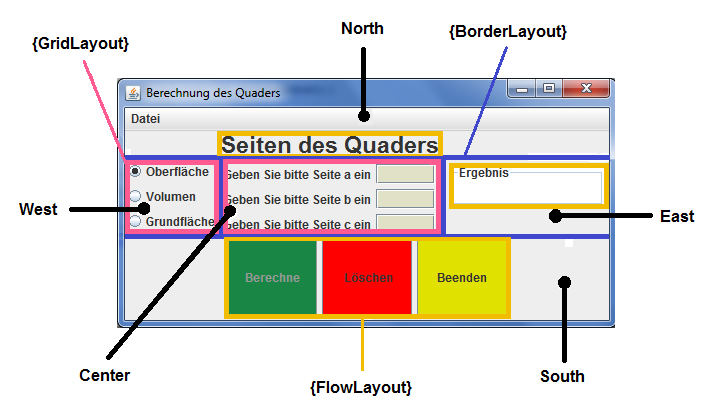
\includegraphics[width=0.8\textwidth]{LayoutTypen.png}
    \caption[Layout-Typen]{Verschiedene Layout-Typen und Positionen eines Layout-Managers}[\cite{Layout}]
\end{figure}
\noindent 
Ein weiteres Feature ist das bei GUI-Frameworks integrierte Event-Handling, welches von großem Vorteil ist, da hiermit, durch vordefinierte Ereignisse wie einen Mausklick ein mögliches Verhalten nach dem Drücken eines Buttons einfach programmiert werden kann.
Nachfolgend werden nun die Frameworks WinForms und WPF vorgestellt.

\subsection{Windows Forms}

Windows Forms\footnote[1]{\cite[Vgl.][]{WindowsForms1}}, kurz WinForms ist eines der beiden bekanntesten GUI-Frameworks von Microsoft. Es gehört, genau wie das später behandelte WPF-Framework zum Microsoft 
.NET Framework.
\\
\begin{figure}[H]
    \centering
    \includegraphics[width=0.2\textwidth]{.NET-Logo.png}
    \caption[.Net-Logo]{Logo von Microsoft .NET}[\cite{DotNet}]
\end{figure}
\noindent
WinForms wurde am 13. Februar 2002 veröffentlicht und bietet einen übersichtlichen Designer mit einer großen Auswahl an Steuerelementen sowie ein umfangreiches Event-Handling. Hiermit lässt sich mit der Programmiersprachen C\# eine Desktop-Anwendung im bekannten und gewohnten Stil von Windows erstellen.\footnote[2]{\cite[Vgl.][]{WindowsForms2}}
\\
\begin{figure}[H]
    \centering
    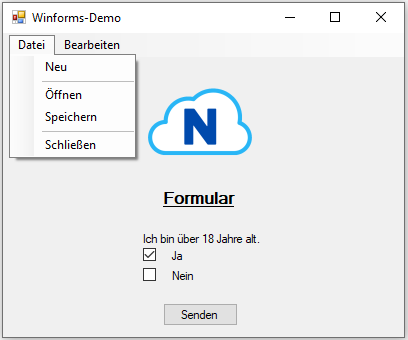
\includegraphics[width=0.5\textwidth]{Winforms-Demo.png}
    \caption{Einfache GUI mit WinForms} 
\end{figure}

\subsection{Windows Presentation Foundation}
Die Windows Presentation Foundation\footnote[3]{\cite[Vgl.][]{WPF1}}, kurz WPF, ist das zweite bekannte Microsoft-Framework zur Erstellung von grafischen Benutzeroberflächen. Die auch unter dem Codenamen Avalon bekannte Klassenbibliothek erschien vier Jahre nach Windows Forms, und zwar im November 2006 im Zuge der neuen .Net-Version 3.0. Im Gegensatz zu WinForms werden in WPF Element wie Buttons, Menüs und weiteres üblicherweise nicht in Programmcode wie C\# definiert sondern mit der auf XML-basierenden Extensible Application Markup Language, kurz XAML.\footnote[4]{\cite[Vgl.][]{WPF2}}

\subsubsection{Extensible Markup Language}
Die sogenannte Extensible Markup Language, ist eine Auszeichnungssprache mit der man Daten in einer hierarchisch strukturierten Form, gespeichert als Textdatei darstellen kann. Diese wurde im Jahr 1998 vom World Wide Web Consortium veröffentlicht und hat den großen Vorteil, dass die geschriebenen Daten sowohl von einem Mensch als auch von einem Computer gelesen werden kann. XML besteht genauso wie HTML, das vor allem für die Erstellung von Webseiten benutzt wird, aus sogenannten Tags welche in Form von spitzen Klammern dargestellt werden. Diese Tags können ineinander verschachtelt sein sowie Parameter besitzen.\footnote[1]{\cite[Vgl.][]{XML}}
\\ \ \\
Die Auszeichnungssprache XAML ist eine eigens von Microsoft entwickelte Version von XML, welche im Zuge von und für WPF entwickelt wurde. Somit können GUI-Elemente wie in HTML einfach erstellt, beliebig angepasst und bearbeitet werden.\footnote[2]{\cite[Vgl.][]{XAML1}}
\\
\begin{figure}[H]
    \centering
    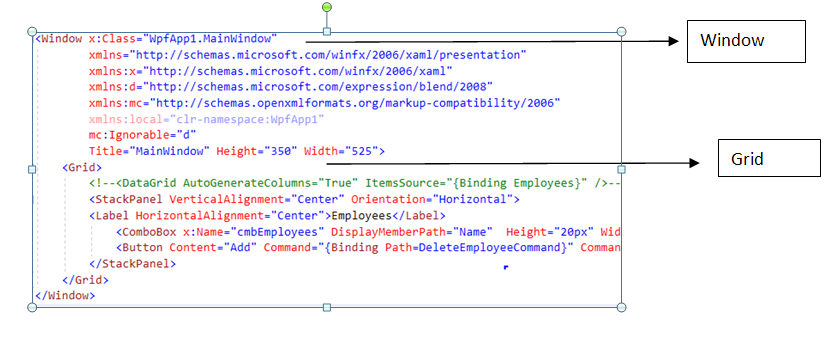
\includegraphics[width=1\textwidth]{Wpf.png}
    \caption[XAML-Code]{Erstellen einer GUI in WPF mit XAML}[\cite{XAML2}]
\end{figure}

\subsection{Vergleich beider GUI-Frameworks}

Einer der größten Nachteile von WinForms gegenüber WPF ist, dass man sich bei der Wahl der Elemente einer GUI nur von den Standard-Windows-Bedienelementen bedienen kann. Möchte man sich also bei der Gestaltung seiner Benutzeroberfläche kreativ ausleben und zum Beispiel einen Button mit runden Ecken einbauen, so stößt man bei WinForms schnell an seine Grenzen, da es schlicht und einfach standardmäßig keinen Button mit runden Ecken in Windows gibt. Im Gegensatz dazu ist WPF nicht von den Standard-Bedienelementen von Windows abhängig und es ist so möglich Elemente in fast allen Formen mit fast jeder bedenklichen Funktionalität zu kreieren. Die scheinbar grenzenlosen Möglichkeiten des GUI-Designens mit WPF können aber auch schnell zu einem Nachteil werden, denn durch die hohe Flexibilität ist es oftmals schwieriger und zeitaufwändiger ein einfaches Element zu erstellen, als es mit WinForms wäre.\footnote[3]{\cite[Vgl.][]{Vergleich}}

\subsection{Einbinden von Dynamic Link Libraries}

 Um das Problem, das man bei der Auswahl der Elemente auf die Standard-Windows-Benutzerelemente beschränkt ist zumindest größtenteils zu beheben, kann man in Visual Studio sogenannte Dynamic Link Libraries, kurz DLL, einbinden. Eine .dll-Datei ist eine Programmbibliothek also eine Sammlung von mehreren Funktionen, welche man bei Bedarf im Hauptprogramm verwenden kann.\footnote[1]{\cite[Vgl.][]{DLL}}

\subsubsection{MetroSuite DLL}

\begin{figure}[H]
    \centering
    
\includegraphics[width=0.5\textwidth]{MetroSuite-Logo.png}
    \caption[MetroSuiteDLL-Logo]{Logo der MetroSuite DLL}[\cite{MetroSuite1}]
\end{figure}
\noindent 
Zur Umsetzung des Designs verwenden wir die MetroSuite DLL\footnote[2]{\cite[Vgl.][]{MetroSuite2}}. Mithilfe dieser ist es möglich, überarbeitete Steuerelemente oder komplett neue Komponenten in die Desktop-Anwendung einzubauen. Ein Beispiel hierfür wäre ein Button mit abgerundeten Ecken oder Animationen bei einem Mausklick auf diesen. Die MetroSuite DLL wurde von Martin Gather implementiert und steht für die nicht kommerzielle Verwendung kostenlos zur Verfügung. Aufgrunddessen, dass sich hiermit fast alle Vorstellungen umsetzen lassen, haben wir uns gegen eine kostenpflichtige Alternative und somit für MetroSuite entschieden.

\section{Grafiksoftware}

Für die visuelle Gestaltung rund um die Desktop-Anwendung benötigen wir zusätzliche Grafiksoftware, welche nachfolgend vorgestellt wird.

\subsection{Figma}

Um die Ideen rund um das Design der Desktop-Anwendung in ein sichtbares Ergebnis umzuwandeln, benutzen wir den webbasierten Vektorgrafik-Editor Figma. Dieses Tool ermöglicht es schnell und unkompliziert Mockups zu kreieren. Dabei bietet es eine Vielzahl an vorgefertigten Formen, Schriften, Icons und weitere Elemente die in einer Desktop-Anwendung nicht fehlen dürfen. Der große Vorteil von Figma ist, dass alle erstellten Grafiken im SVG-Format exportiert werden können. Somit können wir das Tool nicht nur für das Prototyping sondern auch zum Erstellen von Design-Elementen, welche in WinForms importiert werden können, nutzen.\footnote[3]{\cite[Vgl.][]{Figma}}

\subsection{GIMP}

Neben Figma benutzen wir auch das Grafikprogramm GNU Image Manipulation Program, kurz GIMP. Die am 15. Februar 1996 veröffentlichte Software ist eine der bekanntesten Bildbearbeitungsprogramme, welche im Gegensatz zum Marktführer Photoshop kostenfrei zu benutzen ist. Mithilfe von GIMP kann man beispielsweise Logos oder andere Grafiken kreieren.\footnote[1]{\cite[Vgl.][]{GIMP}}

\section{Notification Area}
Als Notification Area werden alle rechtsbündigen Symbole bis zu dem Pfeil, der nach oben zeigt bezeichnet, wenn man auf den Pfeil klickt wird die Overflow Area geöffnet. In diesen Bereich werden standardmäßig einige Symbole verschoben. Jedes Symbol kann von der Notification Area in die Overflow Area verschoben werden dasselbe gilt auch für die andere Richtung.\footnote[1]{\cite[Vgl.][]{10}}
\begin{figure}[H]
    \centering
    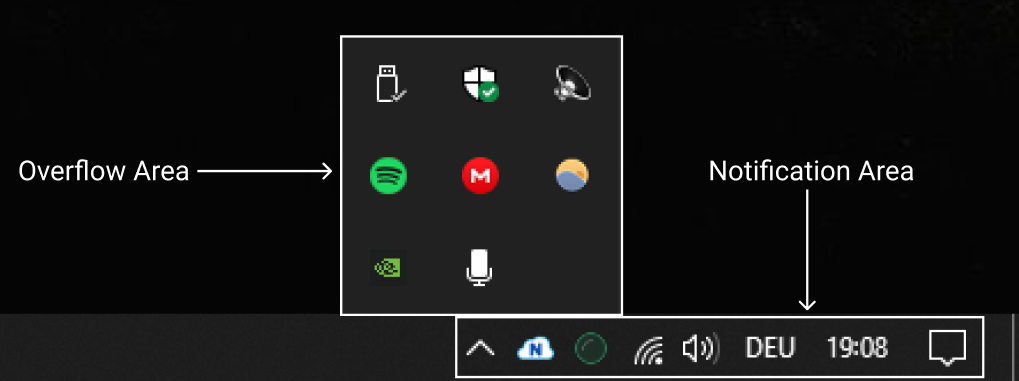
\includegraphics[width=0.8\textwidth]{NotificationArea.png}
    \caption[NotificationArea]{Notification Area} 
\end{figure}
\noindent
Die Notification Area ist besser bekannt unter dem Namen Systemtray, wird aber offiziell von Windows als Notification Area bezeichnet. Der Begriff Systemtray kommt von Windows 95, weil es da eine Anwendung gibt die systray.exe heißt. Nachdem dieses Programm geschlossen wurde, sind die Symbole die in der Notification Area angezeigt wurden verschwunden. Deshalb hat man angenommen, da die Anwendung die dafür zuständig ist systray.exe heißt. Der Name des Bereichs wo die Symbole angezeigt werden Systemtray ist. Das ist aber nicht der einzige Grund der Verwirrung gewesen. Microsoft Mitarbeiter haben den Bereich als Systemtray bezeichnet und bis 2003 war auch in der Windows Dokumentation der Begriff Systemtray enthalten. Nicht nur in der Dokumentation ist Windows so ungenau, auch in den Windows 10 Einstellungen, wenn man seine Systemsprache auf Englisch hat, findet man noch den Begriff Systemtray unter Settings → Ease of Access → Narrator.\footnote[1]{\cite[Vgl.][]{15}}

\subsection{Windows Guidelines}
Dieser Bereich wurde Notification Area genannt, da der Plan war das nur Symbole gezeigt werden, die dem Benutzer hilfreiche Informationen geben entweder anhand von Benachrichtigungen oder das sich das Symbol ändert wie zum Beispiel bei der Akkustandanzeige. Ein anderer wichtiger Aspekt eines Symbols in der Notification Area ist, das die Information wichtig genug sind um den Benutzer zu stören, trotzdem aber keine sofortige  Benutzeraktion erfordert. Die Benachrichtigungen sollen ohne weiteres einfach ignoriert werden können, falls diese Benachrichtigung sofortige Benutzeraktion benötigt, wird einem vorgeschlagen, statt dieser eine Dialog Box zu benutzen. Damit wird der Benutzer dazu gezwungen etwas zu machen, wenn er seinen Computer weiter verwenden will. Es soll möglich sein die Benachrichtigungen auszuschalten. Am besten werden Benutzer nicht von ihrer Arbeit durch die Benachrichtigungen abgelenkt, sondern sehen diese erst, wenn sie schon aus einem anderen Grund den Fokus verloren haben. Viele Entwickler nutzen die Notification Area aber nicht so wie es von Windows selbst vorgeschlagen wird, sondern einfach um ihre Anwendung offenzuhalten, ohne das der normale Benutzer etwas davon weiß.\footnote[2]{\cite[Vgl.][]{17}}